%%%%%%%%%%%%%%%%%%%%%%%%%%%%%%%%%%%%%%%%%%%%%%%%%%%%%%%%%%%%%%%%%%%%%%%%%%%%%%%
%% SOCIOL 723 -- Social Statistics II
%% Week 4: Maximum Likelihood -- Applications (Generalized Linear Models)
%% Wenhao Jiang, Duke University, Fall 2026
%%%%%%%%%%%%%%%%%%%%%%%%%%%%%%%%%%%%%%%%%%%%%%%%%%%%%%%%%%%%%%%%%%%%%%%%%%%%%%%

\documentclass[aspectratio=169,11pt,xcolor=dvipsnames]{beamer}
\mode<presentation>

\usepackage[T1]{fontenc}
\usepackage{lmodern}
\usefonttheme{serif}
\renewcommand{\familydefault}{\rmdefault}

\usepackage{amsmath,amsfonts,amssymb,bm}
\usepackage{graphicx}
\usepackage{booktabs}
\usepackage{tikz}
\usetikzlibrary{arrows.meta,positioning,calc}
\usepackage[english]{babel}

\newcommand{\srcp}[1]{{\scriptsize\color{gray}(#1)}}
\newcommand{\srct}[1]{#1}

\DeclareMathOperator*{\argminop}{arg\,min}
\DeclareMathOperator*{\argmaxop}{arg\,max}
%% \limits forces the subscript underneath even in inline math
\newcommand{\argmin}{\argminop\limits}
\newcommand{\argmax}{\argmaxop\limits}
\DeclareMathOperator{\Cov}{Cov}
\DeclareMathOperator{\Var}{Var}
\DeclareMathOperator{\logit}{logit}
\DeclareMathOperator{\plim}{plim}
\newcommand{\indep}{\perp\!\!\!\perp}

\newcommand{\E}{E}
\newcommand{\En}{\mathbb{E}_n}
\newcommand{\R}{\mathbb{R}}
\newcommand{\X}{\bm{X}}
\newcommand{\Y}{\bm{y}}
\newcommand{\bhat}{\hat{\bm{\beta}}}
\newcommand{\zero}{\bm{0}}
\newcommand{\Ix}{\bm{I}}
\newcommand{\dto}{\overset{d}{\longrightarrow}}
\newcommand{\pto}{\overset{p}{\longrightarrow}}
\newcommand{\lik}{\mathcal{L}}
\newcommand{\loglik}{\ell}
\newcommand{\Info}{\mathcal{I}}
\newcommand{\SE}{\mathrm{se}}

\usetheme{default}
%% thin single-line header: clickable section names, current one highlighted.
%% (miniframes is deliberately not used: one dot per slide wraps to 4 rows here)
\setbeamerfont{section in head/foot}{size=\tiny}
\setbeamertemplate{headline}{%
  \begin{beamercolorbox}[wd=\paperwidth,ht=2.4ex,dp=1.1ex,%
                         leftskip=.3cm,rightskip=.3cm]{section in head/foot}%
    \usebeamerfont{section in head/foot}%
    \insertsectionnavigationhorizontal{.94\paperwidth}{}{}%
  \end{beamercolorbox}%
}

\definecolor{dukeblue}{RGB}{1,33,105}
\definecolor{accent}{RGB}{200,78,0}
\definecolor{softgray}{RGB}{242,242,245}

\setbeamercolor{structure}{fg=dukeblue}
\setbeamercolor{frametitle}{fg=dukeblue,bg=white}
\setbeamercolor{section in head/foot}{fg=white,bg=dukeblue}
\setbeamercolor{section in head/foot shaded}{fg=white!50!dukeblue,bg=dukeblue}
\setbeamercolor{alerted text}{fg=accent}
\setbeamercolor{block title}{fg=white,bg=dukeblue}
\setbeamercolor{block body}{fg=black,bg=softgray}
\setbeamercolor{block title alerted}{fg=white,bg=accent}
\setbeamercolor{block body alerted}{fg=black,bg=softgray}

\setbeamertemplate{footline}[page number]
\setbeamertemplate{navigation symbols}{}
%% continued frames keep the SAME font size and spill onto a new slide
\setbeamertemplate{frametitle continuation}{\ifnum\insertcontinuationcount>1\normalfont\footnotesize\ (cont.)\fi}
\setbeamertemplate{itemize items}[circle]
\setbeamertemplate{blocks}[rounded][shadow=false]
\setbeamerfont{frametitle}{series=\bfseries}
\setbeamerfont{footnote}{size=\scriptsize}
\setbeamerfont{caption}{size=\footnotesize}
\setbeamertemplate{subsection in head/foot}{}
\setbeamertemplate{subsection in head/foot shaded}{}
\setbeamertemplate{caption}[numbered]

\newcommand{\adv}{\,\raisebox{0.6pt}{\textcolor{accent}{$\bigstar$}}}
%% marker for essential material every student must understand (examinable core)
\definecolor{corestar}{RGB}{0,83,155}
\newcommand{\core}{\,\raisebox{0.6pt}{\textcolor{corestar}{$\bigstar$}}}

\setbeamertemplate{section page}{%
  \begin{centering}\vfill
  {\usebeamercolor[fg]{structure}\Large\bfseries\insertsectionhead\par}
  \vskip4pt{\color{dukeblue}\rule{0.35\linewidth}{1pt}\par}
  \vfill\end{centering}}
\setbeamertemplate{subsection page}{%
  \begin{centering}\vfill
  {\usebeamercolor[fg]{structure}\large\bfseries\insertsubsectionhead\par}
  \vfill\end{centering}}

\AtBeginDocument{%
  \setlength{\abovedisplayskip}{5pt}%
  \setlength{\belowdisplayskip}{5pt}%
  \setlength{\abovedisplayshortskip}{2pt}%
  \setlength{\belowdisplayshortskip}{3pt}%
}
\setbeamertemplate{frametitle}{%
  \vskip4pt\usebeamerfont{frametitle}\usebeamercolor[fg]{frametitle}%
  \insertframetitle\par\vskip2pt}
\setbeamersize{text margin left=0.75cm, text margin right=0.75cm}

%% ---- title page: same face as the body (Latin Modern), larger and bold
\setbeamerfont{title}{size*={16}{19},series=\bfseries}
\setbeamerfont{subtitle}{size=\Large,series=\mdseries}
\setbeamerfont{author}{size=\large}
\setbeamerfont{date}{size=\large}
\title[SOCIOL 723]{SOCIOL 723: Social Statistics II\\[-2pt]}
\subtitle{Week 4, Maximum Likelihood: Applications\\[-6pt]}
\author[Jiang]{Wenhao Jiang\vspace{-2.5em}}
\institute[Duke]{}
\titlegraphic{
\includegraphics[height=1.3cm]{../Misc/duke_logo.png}}
\date{Department of Sociology, Fall 2026}

\begin{document}

\begin{frame}[plain]
  \titlepage
\end{frame}

\begin{frame}{Today}
  \tableofcontents
  \vskip6pt
  {\footnotesize Stars: \core{} examinable; \adv{} never examined.}
\end{frame}

%%%%%%%%%%%%%%%%%%%%%%%%%%%%%%%%%%%%%%%%%%%%%%%%%%%%%%%%%%%%%%%%%%%%%%%%%%%%%%%
\section[X inside theta]{Putting $X$ Inside $\theta$}
%%%%%%%%%%%%%%%%%%%%%%%%%%%%%%%%%%%%%%%%%%%%%%%%%%%%%%%%%%%%%%%%%%%%%%%%%%%%%%%
\begin{frame}\sectionpage\end{frame}

\begin{frame}{Where Week 3 Left Us\core}
One parameter $\theta$, one curve $\loglik(\theta)$, and everything read
off that curve:
\begin{itemize}\itemsep3pt
  \item the \textbf{peak} is the estimate $\hat\theta$;
  \item the \textbf{curvature} at the peak, i.e., the second-order
        derivative, is the information; one over its square root is the
        standard error;
  \item a null $\theta_0$ is tested by how far it is from the peak: the
        \textbf{gap} in SE units (Wald, $z^2$) or the \textbf{drop} in
        $\loglik$, doubled (LR). On a parabola they agree; when they
        disagree, believe LR;
  \item models are compared by LR when nested, by BIC when not.
\end{itemize}
\vskip4pt
\textbf{Today.} $\theta$ was the same for everyone. Regression gives
\alert{each person their own $\theta_i$}, built from $X_i$: keep Week 3's
likelihood, substitute $\theta_i = h(X_i'\bm\beta)$, and estimate,
standard errors, and tests carry over. The new work: choosing $h$ and
reading the result.
\end{frame}

\begin{frame}{One $\theta$ for Everyone Is Not a Regression\core}
Week 3's Bernoulli gives every respondent the same $\theta$, the share
with a degree. A regression lets $\theta_i$ depend on $X_i$. First try:
Week 1's line, $\theta_i = \beta_0 + \beta_1 X_i$.
\begin{columns}[c]
\begin{column}{0.54\textwidth}
\centering
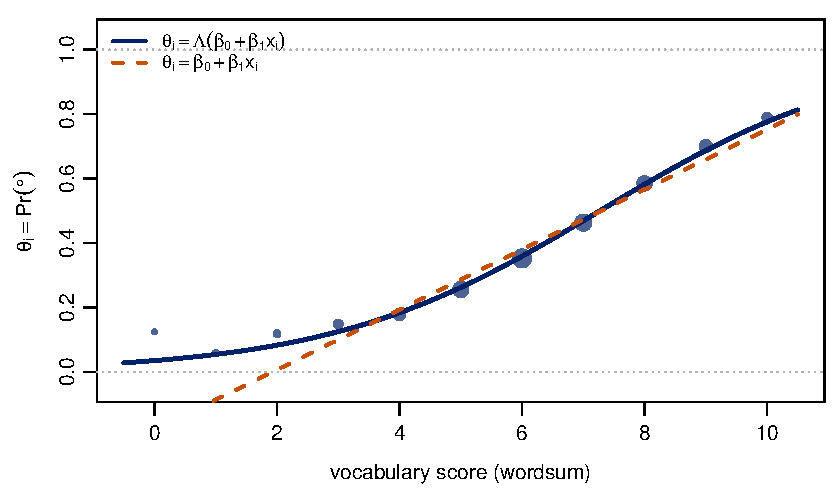
\includegraphics[width=\linewidth]{figs/logit_wordsum.pdf}
\end{column}
\begin{column}{0.44\textwidth}
{\small GSS: share holding a bachelor's degree by vocabulary score (dot
size $=$ number of respondents).}
\begin{itemize}\itemsep3pt
  \item The line reaches $\theta_i < 0$ below a score of $2$. With four
        covariates, $140$ of $3{,}509$ fitted ``probabilities'' fall
        outside $[0, 1]$.
  \item The dots bend. The line cannot.
\end{itemize}
\end{column}
\end{columns}
\vskip2pt
For a rate the same problem: $\theta_i = X_i'\beta$ goes negative, and a
Poisson with a negative rate is not a distribution.
\end{frame}

\begin{frame}{The Fix: a Function With the Right Range\core}
Keep the line $X_i'\bm\beta$ and pass it through a function whose
\emph{output} lives where $\theta$ must:
\begin{center}\small
\renewcommand{\arraystretch}{1.0}
\begin{tabular}{llll}
\toprule
Week 3 model & its $\theta$ lives in & $\theta_i = h(X_i'\bm\beta)$ & the regression \\
\midrule
Normal, mean $\mu$ & $(-\infty, \infty)$ & $\mu_i = X_i'\bm\beta$ & OLS (the hook) \\
Bernoulli, prob.\ $p$ & $(0, 1)$ & $p_i = \Lambda(X_i'\bm\beta) = e^{X_i'\bm\beta}/(1+e^{X_i'\bm\beta})$ & logit \\
Bernoulli, prob.\ $p$ & $(0, 1)$ & $p_i = \Phi(X_i'\bm\beta)$ & probit \\
Poisson, rate $\theta$ & $(0, \infty)$ & $\theta_i = e^{X_i'\bm\beta}$ & Poisson regression \\
\bottomrule
\end{tabular}
\end{center}
\vskip2pt
\begin{itemize}\itemsep2pt
  \item $\Lambda$ and $\Phi$ are S-curves from $0$ to $1$ (the logistic
        and normal CDFs); $e^{(\cdot)}$ is positive.
  \item The \textbf{link function} is the inverse, $g = h^{-1}$, mapping
        $\theta$ back to the line: $g(p) = \log\frac{p}{1-p}$,
        $g(\theta) = \log\theta$. Textbooks start from $g$; think in $h$.
  \item Every row is a \emph{generalized linear model}: a Week 3
        distribution, a line, and an $h$ between them.
\end{itemize}
\end{frame}

\begin{frame}{What Each Regression Is Doing, in Week 3's Terms\core}
Substitute $\theta_i = h(X_i'\bm\beta)$ into Week 3's log-likelihood:
\begingroup
\setlength{\abovedisplayskip}{2pt}\setlength{\belowdisplayskip}{2pt}
\begin{align*}
  \loglik(\bm\beta) = \sum_{i=1}^n \log f\big(y_i \mid \theta_i\big),
  \qquad \theta_i = h(X_i'\bm\beta) .
\end{align*}
\endgroup
\begin{itemize}\itemsep3pt
  \item \textbf{Estimate}: the peak, in $k$ dimensions. No closed form
        except OLS; Newton--Raphson, which \texttt{glm()} runs in a few
        steps.
  \item \textbf{Standard errors}: the curvature at the peak, inverted.
        \texttt{summary()} prints the square roots.
  \item \textbf{Tests}: \texttt{summary()}'s $z$ is Wald; \texttt{anova()}
        is LR.
  \item \textbf{Comparison}: AIC and BIC from $\loglik(\hat{\bm\beta})$.
\end{itemize}
\vskip3pt
\alert{The only new work is interpretation.} $\beta_j$ moves the line; how
much it moves $\theta_i$ depends on $h$ and on where person $i$ sits.
\end{frame}

%%%%%%%%%%%%%%%%%%%%%%%%%%%%%%%%%%%%%%%%%%%%%%%%%%%%%%%%%%%%%%%%%%%%%%%%%%%%%%%
\section[Binary]{Binary Outcomes}
%%%%%%%%%%%%%%%%%%%%%%%%%%%%%%%%%%%%%%%%%%%%%%%%%%%%%%%%%%%%%%%%%%%%%%%%%%%%%%%
\begin{frame}\sectionpage\end{frame}

\begin{frame}{The Logit Model, Written Two Ways\core}
Two ways to write the same model, the textbook's and the last section's:
\begingroup
\setlength{\abovedisplayskip}{2pt}\setlength{\belowdisplayskip}{2pt}
\begin{align*}
  \log\tfrac{p_i}{1-p_i} &= X_i'\bm\beta
    && \text{\footnotesize textbook form: log-odds linear in $X$} \\
  \tfrac{p_i}{1-p_i} &= e^{X_i'\bm\beta}
    && \text{\footnotesize exponentiate both sides} \\
  p_i &= e^{X_i'\bm\beta} - e^{X_i'\bm\beta}\,p_i
    && \text{\footnotesize multiply by $1 - p_i$} \\
  p_i\,\big(1 + e^{X_i'\bm\beta}\big) &= e^{X_i'\bm\beta}
    && \text{\footnotesize collect the $p_i$ terms} \\
  p_i &= \tfrac{e^{X_i'\bm\beta}}{1 + e^{X_i'\bm\beta}} = \Lambda(X_i'\bm\beta)
    && \text{\footnotesize divide: probability form}
\end{align*}
\endgroup
\begin{itemize}\itemsep2pt
  \item Every step reverses: the forms are equivalent, and $\Lambda$ is
        the inverse of the log-odds. Read coefficients on the first line
        ($\beta_j$ adds to the log-odds, $e^{\beta_j}$ multiplies the
        odds); compute on the last.
  \item Also from line 2: $1 - p_i = 1/(1 + e^{X_i'\bm\beta})$, used next.
\end{itemize}
\end{frame}

\begin{frame}{The S-Curve\core}
\begin{columns}[c]
\begin{column}{0.46\textwidth}
\centering
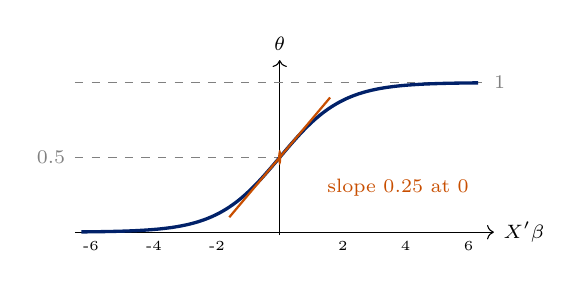
\begin{tikzpicture}[x=0.40cm,y=1.9cm]
  \draw[->] (-6.5,0) -- (6.8,0) node[right]{\scriptsize $X'\beta$};
  \draw[->] (0,-0.02) -- (0,1.15) node[above]{\scriptsize $\theta$};
  \draw[gray,dashed] (-6.5,1) -- (6.5,1) node[right]{\scriptsize 1};
  \draw[gray,dashed] (-6.5,0.5) -- (0,0.5);
  \node[gray,left] at (-6.5,0.5) {\scriptsize 0.5};
  \draw[dukeblue,very thick,smooth,samples=90,domain=-6.3:6.3,variable=\x]
    plot ({\x},{1/(1+exp(-\x))});
  \draw[accent,thick] (-1.6,0.1) -- (1.6,0.9);
  \fill[accent] (0,0.5) circle (0.05);
  \node[accent,anchor=west] at (1.2,0.3) {\scriptsize slope $0.25$ at $0$};
  \foreach \t in {-6,-4,-2,2,4,6} \node[below] at (\t,0) {\tiny \t};
\end{tikzpicture}
\end{column}
\begin{column}{0.52\textwidth}
\begin{itemize}\itemsep2pt
  \item $\Lambda$ is an S-curve: flat near $0$ and $1$, steepest at
        $X'\beta = 0$ where $\theta = 0.5$ (slope $0.25$). Any real
        $X'\beta$ lands inside $(0, 1)$.
  \item The slope at a person's $X'\beta$ is $\theta(1-\theta)$: one
        unit of $X'\beta$ moves the probability by up to $0.25$ in the
        middle and almost nothing in the tails.
  \item Only $0$s and $1$s are observed on the vertical axis; the
        likelihood estimates the curve from them.
\end{itemize}
\end{column}
\end{columns}
\end{frame}

\begin{frame}{The Logit Model, and One Fitted to the GSS\core}
Week 3's Bernoulli log-likelihood with $p_i = \Lambda(X_i'\bm\beta)$
substituted:
\begingroup
\setlength{\abovedisplayskip}{2pt}\setlength{\belowdisplayskip}{2pt}
\begin{align*}
  \loglik(\bm\beta) = \sum_{i=1}^{n}\Big[\, y_i \log p_i + (1-y_i)\log(1-p_i)\Big]
  = \sum_{i=1}^{n}\Big[\, y_i\, X_i'\bm\beta - \log\big(1+e^{X_i'\bm\beta}\big)\Big]
\end{align*}
\endgroup
{\footnotesize (second form: $\log\frac{p_i}{1-p_i} = X_i'\bm\beta$,
$\log(1-p_i) = -\log(1+e^{X_i'\bm\beta})$; concave, so the peak is unique
when it exists.) Holding a bachelor's degree, $n = 3{,}509$:}
\begin{center}\small
\renewcommand{\arraystretch}{1.05}
\begin{tabular}{lrrrr}
\toprule
 & $\hat\beta$ & SE & $z$ & $e^{\hat\beta}$ \\
\midrule
intercept & $-5.81$ & $0.25$ & $-23.7$ & \\
parents' education (years) & $0.207$ & $0.013$ & $15.4$ & $1.23$ \\
vocabulary score (0--10) & $0.391$ & $0.024$ & $16.3$ & $1.48$ \\
female & $0.279$ & $0.078$ & $3.6$ & $1.32$ \\
black & $-0.114$ & $0.110$ & $-1.0$ & $0.89$ \\
\bottomrule
\end{tabular}
\end{center}
Peak, curvature, Wald ruler: all Week 3. The last column is the
interpretation problem.
\end{frame}

\begin{frame}{Newton by Hand on the GSS: Degree on Vocabulary}
Week 3's Newton step, with a gradient and a curvature matrix:
\begingroup
\setlength{\abovedisplayskip}{2pt}\setlength{\belowdisplayskip}{2pt}
\begin{align*}
  \bm\beta^{[t+1]} = \bm\beta^{[t]} + \Info(\bm\beta^{[t]})^{-1} S(\bm\beta^{[t]}),
  \quad
  S(\bm\beta) = \sum_i (y_i - p_i)X_i,
  \quad
  \Info(\bm\beta) = \sum_i p_i(1-p_i)X_iX_i' .
\end{align*}
\endgroup
Start at $\bm\beta = (0, 0)$, so every $p_i = 0.5$:
\begin{center}\small
\renewcommand{\arraystretch}{1.0}
\begin{tabular}{crrrr}
\toprule
step $t$ & $\beta_0$ & $\beta_1$ & $\loglik$ & score $S = (S_0, S_1)$ \\
\midrule
0 & $0$ & $0$ & $-2432.3$ & $(-313.5,\ -792.5)$ \\
1 & $-2.718$ & $0.373$ & $-2133.4$ & $(-38.8,\ -82.4)$ \\
2 & $-3.272$ & $0.450$ & $-2125.6$ & $(-2.4,\ -5.1)$ \\
3 & $-3.313$ & $0.456$ & $-2125.53$ & $(0.0,\ 0.0)$ \\
\bottomrule
\end{tabular}
\end{center}
\begin{itemize}\itemsep1pt
  \item Three steps and the score is zero: the peak.
        \texttt{glm(ba \~{} wordsum)} reports $(-3.313,\ 0.456)$.
  \item The score says which way is uphill, the curvature matrix how far.
        Inverted at the peak, it is the variance matrix.
\end{itemize}
\end{frame}

\begin{frame}{The Logit Score Is the OLS Normal Equation}
Differentiate, using $\partial\Lambda(z)/\partial z = \Lambda(z)(1-\Lambda(z))$:
\begin{align*}
  \frac{\partial\loglik}{\partial\bm\beta}
  = \sum_{i=1}^n \Big[ y_i X_i - \frac{e^{X_i'\bm\beta}}{1+e^{X_i'\bm\beta}}X_i\Big]
  = \sum_{i=1}^n \big(y_i - p_i\big)X_i \ \overset{!}{=}\ \zero .
\end{align*}
\vskip4pt
\begin{alertblock}{Read it}
$\sum_i (y_i - \hat p_i)X_i = \zero$: the residuals $y_i - \hat p_i$ are
orthogonal to the regressors, \alert{exactly the OLS normal equations} with
the fitted probability in place of the fitted value. The fitted probabilities average to the
sample share, $0.41$. (OLS with an intercept has the same property: $\bar{\hat y} =
\bar y$.)
\end{alertblock}
\vskip3pt
No closed form: Newton, as on the last frame. The curvature
$\Info(\bm\beta) = \sum_i p_i(1-p_i)X_iX_i'$, inverted at $\hat{\bm\beta}$,
is the variance matrix: the SE column.
\end{frame}

\begin{frame}{Three Scales, One Coefficient\core}
Take vocabulary: $\hat\beta = 0.391$.
\begin{center}\small
\renewcommand{\arraystretch}{1.35}
\begin{tabular}{llll}
\toprule
Scale & Quantity & $\hat\beta = 0.391$ says & \\
\midrule
Log-odds & $\log\frac{p}{1-p} = X'\bm\beta$ & one more word adds $0.391$ & linear, not intuitive \\
Odds & $\frac{p}{1-p} = e^{X'\bm\beta}$ & odds multiply by $e^{0.391} = 1.48$ & the \emph{odds ratio} \\
Probability & $p = \Lambda(X'\bm\beta)$ & depends on where you start & \alert{what we care about} \\
\bottomrule
\end{tabular}
\end{center}
\vskip4pt
\begin{itemize}\itemsep3pt
  \item An odds ratio of $1.48$ fits $0.05 \to 0.07$ and $0.40 \to 0.50$
        alike. \alert{It is not a risk ratio and not a difference in
        probabilities}; do not read ``$48\%$ more likely.''
  \item On the probability scale one more word adds
        $\Lambda(\eta + 0.391) - \Lambda(\eta)$: large near $p = 0.5$,
        tiny near $0$ or $1$.
  \item Report on the probability scale, and say \emph{for whom}.
\end{itemize}
\end{frame}

\begin{frame}{Start With Predicted Probabilities\core}
How likely is a degree if your parents finished high school ($12$ years)
rather than college ($16$)? For people like those in the data:
\begin{columns}[c]
\begin{column}{0.46\textwidth}
\centering
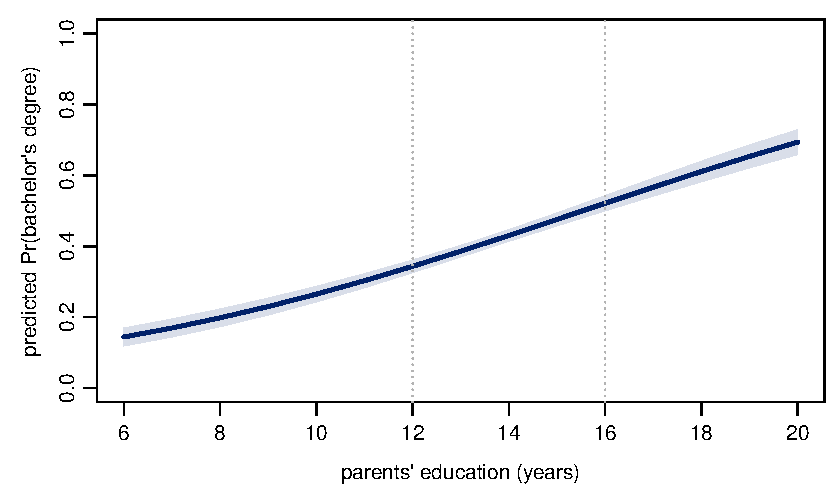
\includegraphics[width=0.76\linewidth]{figs/pred_pareduc.pdf}
\end{column}
\begin{column}{0.52\textwidth}
\begin{center}\small
\renewcommand{\arraystretch}{0.95}
\begin{tabular}{lcc}
\toprule
parents' educ & $\Pr(\text{degree})$ & 95\% CI \\
\midrule
8  & $0.20$ & $[0.17,\ 0.22]$ \\
12 & $0.34$ & $[0.33,\ 0.36]$ \\
16 & $0.52$ & $[0.50,\ 0.54]$ \\
20 & $0.69$ & $[0.66,\ 0.73]$ \\
\bottomrule
\end{tabular}
\end{center}
\end{column}
\end{columns}
\vskip1pt
\begin{itemize}\itemsep2pt
  \item \textbf{Observed-value approach} \srcp{Hanmer and Kalkan 2013}:
        set parents' education to $12$ for \emph{everyone}, keep every
        other covariate at its actual value, compute $\hat p_i$, average;
        repeat at $16$. High school to college: $18$ points.
  \item The standard presentation in sociology journals: a curve with a
        band across the key variable, everything else at observed values;
        coefficients in the appendix. \texttt{avg\_predictions()}.
\end{itemize}
\end{frame}

\begin{frame}{Reading a Logit Slowly: Pager (2003, \emph{AJS})\core}
``The Mark of a Criminal Record.'' Matched testers applied for $350$
jobs; the outcome is a callback ($0/1$); the regressors are
\emph{record}, \emph{Black}, and their product. Appendix table B1:
$\hat\beta_{\text{record}} = -0.99$, $\hat\beta_{\text{Black}} = -1.25$,
interaction $-0.29$. The base cell is white, no record, so
$\hat\beta_0 = -0.66$: odds $e^{-0.66} = 0.52$, probability
$0.52/1.52 = 0.34$, Pager's $34\%$.
\begin{center}\footnotesize
\renewcommand{\arraystretch}{1.05}\setlength{\tabcolsep}{4pt}
\begin{tabular}{lcccc}
\toprule
cell & log-odds $X'\hat\beta$ & odds $e^{X'\hat\beta}$ & $\hat p = \text{odds}/(1+\text{odds})$ & Pager \\
\midrule
white, no record & $-0.66$ & $0.52$ & $0.34$ & $34\%$ \\
white, record & $-0.66 - 0.99 = -1.65$ & $0.19$ & $0.16$ & $17\%$ \\
Black, no record & $-0.66 - 1.25 = -1.91$ & $0.15$ & $0.13$ & $14\%$ \\
Black, record & $-0.66 - 0.99 - 1.25 - 0.29 = -3.19$ & $0.04$ & $0.04$ & $5\%$ \\
\bottomrule
\end{tabular}
\end{center}
\vskip2pt
Read one column at a time. A coefficient \emph{adds} on the log-odds
scale (column 2); exponentiating turns adding into multiplying (column
3); odds over one plus odds is a probability (column 4), which is what the
audit counted (column 5; the small gaps are Pager's two controls).
\end{frame}

\begin{frame}{The Average Marginal Effect, Person by Person\core}
Person $i$'s slope in vocabulary is $\hat p_i(1-\hat p_i)\times 0.391$.
Four real respondents, then the average over all $3{,}509$:
\begin{center}\footnotesize
\renewcommand{\arraystretch}{1.0}
\begin{tabular}{lcccc}
\toprule
respondent & $X_i'\hat\beta$ & $\hat p_i$ & $\hat p_i(1-\hat p_i)$ & slope $= \hat p_i(1-\hat p_i)\times 0.391$ \\
\midrule
parents 12, voc.\ 1, male, white & $-2.94$ & $0.05$ & $0.048$ & $0.019$ \\
parents 12, voc.\ 6, male, Black & $-1.10$ & $0.25$ & $0.188$ & $0.073$ \\
parents 13, voc.\ 8, male, white & $0.01$ & $0.50$ & $0.250$ & $0.098$ \\
parents 20, voc.\ 8, female, white & $1.73$ & $0.85$ & $0.128$ & $0.050$ \\
\midrule
average over all $3{,}509$ & & & $0.192$ & $\mathbf{0.075}$ = AME \\
one person at the sample means & $-0.49$ & $0.38$ & $0.236$ & $0.092$ = MEM \\
\bottomrule
\end{tabular}
\end{center}
\begin{itemize}\itemsep1pt
  \item Same $0.391$ in every row; what differs is where each person sits
        on the S-curve: the slope peaks at $\hat p = 0.5$ and is a fifth
        of that at $\hat p = 0.05$.
  \item The AME is the average of the last column, equally $0.192 \times
        0.391$. The MEM plugs in the means ($13.2$ years, $6.3$ words,
        $0.48$ female, $0.15$ Black): a person who does not exist, near
        the steep part.
\end{itemize}
\end{frame}

\begin{frame}{Then Marginal Effects: One Number per Variable\core}
Predicted probabilities take a figure per variable. A table wants one
number per variable, comparable across models and papers: the
\textbf{average slope} of that curve.
\begin{itemize}\itemsep3pt
  \item For one person the slope of the probability in $X_j$ is
        $\partial p_i/\partial X_{ij} = p_i(1-p_i)\,\beta_j$: $\beta_j$
        scaled by where the person sits on the S-curve ($0$ to $0.25$).
  \item \textbf{Average marginal effect (AME)}, $0.075$: ``averaged over
        the people in the sample, one more word raises the probability of
        a degree by $7.5$ percentage points.'' The last frame's average.
  \item \textbf{Marginal effect at the mean (MEM)}, $0.092$: ``for one
        hypothetical person at the mean of every covariate, one more word
        adds $9.2$ points.'' Older papers report it; report the AME.
\end{itemize}
\texttt{avg\_slopes(m)} computes all of them.
\end{frame}

\begin{frame}{Uncertainty for These Quantities}
An AME or a predicted probability is a \emph{nonlinear} function of
$\hat{\bm\beta}$; its SE is not in the regression table. Three ways:
\begin{enumerate}\itemsep4pt
  \item \textbf{Delta method}: linearize $g(\hat{\bm\beta})$ and use
        $\nabla g'\,\hat V(\hat{\bm\beta})\,\nabla g$. Analytic, fast, the
        default in \texttt{marginaleffects}. The SEs on the last two frames
        are these.
  \item \textbf{Simulation} \srcp{King, Tomz, and Wittenberg 2000}: draw
        $\tilde{\bm\beta}^{(s)} \sim \mathcal N(\hat{\bm\beta}, \hat V)$,
        recompute the quantity at each draw, take percentiles. Any
        nonlinearity, no calculus.
  \item \textbf{Bootstrap} (Week 2): resample rows, refit, recompute.
        Slowest, fewest assumptions.
\end{enumerate}
\vskip3pt
\alert{Do not} build an interval on the log-odds scale and transform its
endpoints if what you want is an interval for a \emph{difference} in
probabilities.
\end{frame}

\begin{frame}{Probit: Another S-Curve\core}
\begin{columns}[c]
\begin{column}{0.44\textwidth}
\centering
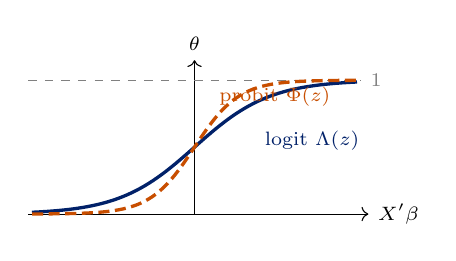
\begin{tikzpicture}[x=0.48cm,y=1.7cm]
  \draw[->] (-4.4,0) -- (4.6,0) node[right]{\scriptsize $X'\beta$};
  \draw[->] (0,0) -- (0,1.15) node[above]{\scriptsize $\theta$};
  \draw[gray,dashed] (-4.4,1) -- (4.4,1) node[right]{\scriptsize 1};
  \draw[dukeblue,very thick,smooth,samples=90,domain=-4.3:4.3,variable=\x]
    plot ({\x},{1/(1+exp(-\x))});
  \draw[accent,very thick,dash pattern=on 4pt off 2pt,smooth,samples=90,domain=-4.3:4.3,variable=\x]
    plot ({\x},{1/(1+exp(-1.702*\x))});
  \node[dukeblue,anchor=west] at (1.6,0.55) {\scriptsize logit $\Lambda(z)$};
  \node[accent,anchor=west] at (0.4,0.88) {\scriptsize probit $\Phi(z)$};
\end{tikzpicture}
\end{column}
\begin{column}{0.54\textwidth}
\begin{itemize}\itemsep3pt
  \item Any function that rises from $0$ to $1$ can play $h$. The
        logistic $\Lambda$ is one; the normal CDF $\Phi$ is the other
        common choice: $p_i = \Phi(X_i'\bm\beta)$, the \textbf{probit}.
  \item $\Phi$ is a slightly narrower S. Stretch its axis by $1.7$ and it
        sits on $\Lambda$ to within $0.01$: same shape, different units.
\end{itemize}
\end{column}
\end{columns}
\begin{center}\small
\renewcommand{\arraystretch}{1.0}
\begin{tabular}{lcccc}
\toprule
 & parents' educ & vocabulary & female & black \\
\midrule
logit $\hat\beta$  & $0.207$ & $0.391$ & $0.279$ & $-0.114$ \\
probit $\hat\beta$ & $0.117$ & $0.233$ & $0.159$ & $-0.070$ \\
ratio & $1.77$ & $1.68$ & $1.75$ & $1.64$ \\
AME, logit / probit & $0.040$ / $0.038$ & $0.075$ / $0.075$ & $0.054$ / $0.052$ & $-0.022$ / $-0.023$ \\
\bottomrule
\end{tabular}
\end{center}
\end{frame}

\begin{frame}{Logit or Probit: a Recommendation\core}
\begin{itemize}\itemsep5pt
  \item \textbf{Default to logit.} It has the cleaner likelihood, odds
        ratios for the audiences that want them, and it is what every
        package and most readers expect.
  \item \textbf{Probit when the next step needs a normal}: selection
        models, bivariate probit, or a subfield convention. Probit comes
        from economics and psychometrics, where it arrived first.
  \item \textbf{Never compare raw coefficients across nested models or
        across groups}, in either model. Adding a covariate rescales all
        the coefficients, even ones whose effect is unchanged
        \srcp{Allison 1999; Mood 2010}. Compare AMEs or predicted
        probabilities, which live on the probability scale.
  \item \textbf{Never agonize.} AMEs from the two agree to two decimals;
        the choice is a footnote.
\end{itemize}
\end{frame}

\begin{frame}{Interactions in Nonlinear Models\core}
Two questions: should the product $X_1 X_2$ be in the model, and do the
models with and without it agree on probabilities? What each can say
about $X_1$'s effect across $X_2$:
\begin{center}\footnotesize
\renewcommand{\arraystretch}{1.1}\setlength{\tabcolsep}{5pt}
\begin{tabular}{lll}
\toprule
 & log-odds scale & probability scale \\
\midrule
no product & one slope, $\beta_1$, forced equal across $X_2$ &
  differs across $X_2$ anyway, by $p_i(1-p_i)$ only \\
with product & $\beta_1 + \beta_{12} X_2$, the data choose $\beta_{12}$ &
  differs by $p_i(1-p_i)$ \emph{and} by $\beta_{12}$ \\
\bottomrule
\end{tabular}
\end{center}
\begin{itemize}\itemsep2pt
  \item \textbf{Include the product} whenever the question is whether
        $X_1$'s effect differs by $X_2$. Without it the answer is fixed in
        advance: zero on the log-odds scale, whatever the S-curve gives on
        the probability scale
        \srcp{Ai and Norton 2003; Berry, DeMeritt, and Esarey 2010}.
  \item \textbf{The two models agree} on probabilities only when
        $\hat\beta_{12} \approx 0$; otherwise the no-product model has the
        wrong probabilities in the cells.
  \item \textbf{Report} the interaction as a difference in AMEs of $X_1$
        between the $X_2$ groups, with an interval. $\hat\beta_{12}$ is on
        the wrong scale for the question.
\end{itemize}
\end{frame}

\begin{frame}{Interactions: Real Output, Number by Number\core}
Does parents' education matter more for women? Add the product:
\texttt{ba \~{} pareduc * female + wordsum + black}.
\begin{columns}[c]
\begin{column}{0.48\textwidth}
\centering\scriptsize
\renewcommand{\arraystretch}{1.0}\setlength{\tabcolsep}{3pt}
\begin{tabular}{lrrr}
\toprule
 & $\hat\beta$ & SE & $z$ \\
\midrule
parents' educ & $0.197$ & $0.018$ & $10.9$ \\
female & $-0.012$ & $0.377$ & $-0.03$ \\
parents' educ $\times$ female & $0.021$ & $0.027$ & $0.79$ \\
\bottomrule
\end{tabular}
\end{column}
\begin{column}{0.50\textwidth}
\centering\scriptsize
\renewcommand{\arraystretch}{1.0}\setlength{\tabcolsep}{3pt}
\begin{tabular}{lcc}
\toprule
AME of parents' educ & no product & with product \\
\midrule
among men & $0.039$ & $0.037$ \\
among women & $0.041$ & $0.043$ \\
difference (SE) & $0.002$ & $0.006$ ($0.004$) \\
\bottomrule
\end{tabular}
\end{column}
\end{columns}
\vskip3pt
\begin{itemize}\itemsep2pt
  \item \textbf{Log-odds scale}: a year of parents' education adds
        $0.197$ for men and $0.197 + 0.021$ for women. The product is not
        significant ($z = 0.79$, LR $= 0.6$).
  \item \textbf{No-product column}: women's AME is already larger,
        $0.041$ against $0.039$, with no product in the model. That gap
        is the S-curve alone: women sit where it is steeper.
  \item \textbf{With-product column}: the gap is $0.006$ per year, SE
        $0.004$. This answers the question; the answer is no. The two
        models nearly agree because $\hat\beta_{12}$ is near zero.
        \texttt{avg\_slopes(m, variables = "pareduc", by = "female")}.
\end{itemize}
\end{frame}

%%%%%%%%%%%%%%%%%%%%%%%%%%%%%%%%%%%%%%%%%%%%%%%%%%%%%%%%%%%%%%%%%%%%%%%%%%%%%%%
\section[Several Categories]{Outcomes With Several Categories}
%%%%%%%%%%%%%%%%%%%%%%%%%%%%%%%%%%%%%%%%%%%%%%%%%%%%%%%%%%%%%%%%%%%%%%%%%%%%%%%
\begin{frame}\sectionpage\end{frame}

\begin{frame}{The Setup: One Outcome, Four Regions\core}
\textbf{The outcome.} Where a respondent lives: Midwest, Northeast,
South, West ($J = 4$). \alert{These categories have no order}: the West
is not ``more'' than the South. That is what makes this the multinomial,
not the ordered, case.
\vskip0pt
\textbf{Week 3's Bernoulli, generalized.} $Y_i$ takes one of $J$ values
with probabilities $p_{i1}, \dots, p_{iJ}$ adding to one:
\begingroup
\setlength{\abovedisplayskip}{2pt}\setlength{\belowdisplayskip}{2pt}
\begin{align*}
  \loglik = \sum_{i=1}^n \sum_{j=1}^J \mathbf 1[Y_i = j]\,\log p_{ij}
  \qquad\text{\footnotesize one nonzero term per person; $J = 2$ is Week 3's Bernoulli.}
\end{align*}
\endgroup
\textbf{The regression.} Four probabilities per person from $X_i$. Pick a
base, the Midwest, and write one logit for every other region
\emph{against the base}:
\begingroup
\setlength{\abovedisplayskip}{2pt}\setlength{\belowdisplayskip}{2pt}
\begin{align*}
  \log\frac{p_{ij}}{p_{i,\text{Midwest}}} = X_i'\bm\beta_j,
  \qquad j = \text{Northeast},\ \text{South},\ \text{West}.
\end{align*}
\endgroup
Three lines, three coefficient vectors. The base gets none: its own line
would read $\log(p_{i,\text{base}}/p_{i,\text{base}}) = 0$; writing
$\bm\beta_{\text{base}} = \bm 0$ is a convention so one formula covers all
four ($e^0 = 1$).
\end{frame}

\begin{frame}{From $J - 1$ Log-Odds to $J$ Probabilities\core}
The same algebra as the two-ways frame, with a sum in the denominator:
\begingroup
\setlength{\abovedisplayskip}{2pt}\setlength{\belowdisplayskip}{2pt}
\begin{align*}
  p_{ij} &= p_{i,\text{base}}\, e^{X_i'\bm\beta_j}
    && \text{\footnotesize exponentiate the $j$th line} \\
  1 = \sum_j p_{ij} &= p_{i,\text{base}}\Big(1 + \sum_{m \ne \text{base}} e^{X_i'\bm\beta_m}\Big)
    && \text{\footnotesize add up all $J$; the base contributes $e^0 = 1$} \\
  p_{i,\text{base}} &= 1\Big/\Big(1 + \sum_{m} e^{X_i'\bm\beta_m}\Big)
    && \text{\footnotesize solve for the base} \\
  p_{ij} &= e^{X_i'\bm\beta_j}\Big/\Big(1 + \sum_{m} e^{X_i'\bm\beta_m}\Big)
    && \text{\footnotesize substitute back: the multinomial logit}
\end{align*}
\endgroup
\begin{itemize}\itemsep2pt
  \item Positive and summing to one by construction. With $J = 2$ this is
        $\Lambda(X_i'\bm\beta)$: the logit is the special case. Estimation
        is Week 3 again, Newton over $(J-1)k = 15$ coefficients;
        \texttt{nnet::multinom}.
  \item \textbf{IIA}: the odds of $j$ versus $m$ never involve a third
        category, so adding an option cannot change the ratio of two old
        ones.
\end{itemize}
\end{frame}

\begin{frame}{Multinomial Logit on the GSS: Where People Live\core}
Base Midwest; each row is one line, shown as $e^{\hat\beta}$ (odds
multipliers), $n = 3{,}509$:
\begin{center}\small
\renewcommand{\arraystretch}{1.0}
\begin{tabular}{lcccc}
\toprule
versus Midwest & education (per year) & Black & female & age (per year) \\
\midrule
Northeast & $1.08$ & $1.32$ & $1.08$ & $1.00$ \\
South & $0.98$ & $\mathbf{2.88}$ & $1.21$ & $1.00$ \\
West & $1.01$ & $0.82$ & $1.13$ & $0.99$ \\
\bottomrule
\end{tabular}
\end{center}
Reading one cell: a Black respondent's odds of living in the South
\emph{rather than the Midwest} are $2.88$ times a white respondent's,
other things equal. Change the base and every number changes, so report
the four probabilities, observed-value style:
\begin{center}\small
\renewcommand{\arraystretch}{1.0}
\begin{tabular}{lcccc}
\toprule
 & Midwest & Northeast & South & West \\
\midrule
not Black & $0.26$ & $0.17$ & $0.33$ & $0.23$ \\
Black & $0.16$ & $0.14$ & $0.58$ & $0.12$ \\
\bottomrule
\end{tabular}
\end{center}
Education moves people toward the Northeast ($0.14 \to 0.18$, 12 to 16
years) and out of the South ($0.40 \to 0.35$). All $12$ slopes: $LR = 171$.
\end{frame}

\begin{frame}{How the Four Probabilities Are Computed\core}
\textbf{Step 1: one person, one setting.} A respondent with $16$ years
of education, female, aged $40$, Black \emph{set} to $1$. One linear
predictor per non-base line, then the formula:
\begin{center}\small
\renewcommand{\arraystretch}{1.0}
\begin{tabular}{lcccc}
\toprule
 & Midwest (base) & Northeast & South & West \\
\midrule
$X_i'\hat{\bm\beta}_j$ & $0$ & $0.011$ & $1.352$ & $-0.196$ \\
$e^{X_i'\hat{\bm\beta}_j}$ & $1$ & $1.011$ & $3.867$ & $0.822$ \\
$\hat p_{ij} = e^{X_i'\hat{\bm\beta}_j}/6.70$ & $0.149$ & $0.151$ & $0.577$ & $0.123$ \\
\bottomrule
\end{tabular}
\end{center}
The denominator $6.70 = 1 + 1.011 + 3.867 + 0.822$ is shared by the four
cells, which is why they add to one. Set Black $= 0$ for the same person
and the row becomes $0.243,\ 0.186,\ 0.327,\ 0.244$.
\vskip2pt
\textbf{Step 2: everyone, then average.} Repeat step 1 for all $3{,}509$
respondents with Black set to $1$, each keeping their own education,
gender, and age; average each column: $0.16,\ 0.14,\ 0.58,\ 0.12$. Then
with Black set to $0$: $0.26,\ 0.17,\ 0.33,\ 0.23$. Those are the last
frame's two rows. \texttt{avg\_predictions(m, variables = "black")}.
\end{frame}

\begin{frame}{Ordered Logit: Using the Order\core}
Degree is ordered; a multinomial on it would spend $20$ parameters
ignoring that. Use the order: model the probability of being \emph{at or
below} each level,
\begingroup
\setlength{\abovedisplayskip}{2pt}\setlength{\belowdisplayskip}{2pt}
\begin{align*}
  \log\frac{\Pr(Y_i \le j)}{\Pr(Y_i > j)} = \tau_j - X_i'\bm\beta,
  \quad j = 1, \dots, J-1
  \qquad\Longrightarrow\qquad
  \Pr(Y_i \le j) = \Lambda(\tau_j - X_i'\bm\beta),
\end{align*}
\endgroup
one $\bm\beta$ for every cut and $J - 1$ thresholds $\tau_1 < \cdots <
\tau_{J-1}$: $4 + 4 = 8$ parameters. Category probabilities are
differences of neighbouring cumulative ones, $p_{ij} = \Lambda(\tau_j -
X_i'\bm\beta) - \Lambda(\tau_{j-1} - X_i'\bm\beta)$. Larger $X_i'\bm\beta$
pushes probability up the ladder.
\begin{center}\small
\renewcommand{\arraystretch}{1.0}
\begin{tabular}{lrr@{\qquad}lr}
\toprule
 & $\hat\beta$ & $z$ & cutpoint & $\hat\tau$ \\
\midrule
parents' education & $0.208$ & $19.9$ & $<$HS $\mid$ HS & $1.84$ \\
vocabulary & $0.358$ & $18.6$ & HS $\mid$ junior college & $5.21$ \\
female & $0.335$ & $5.2$ & junior college $\mid$ bachelor's & $5.67$ \\
black & $-0.024$ & $-0.3$ & bachelor's $\mid$ graduate & $7.36$ \\
\bottomrule
\end{tabular}
\end{center}
$\hat\beta$ reads like a logit coefficient; the cutpoints are the
intercepts. \texttt{MASS::polr}.
\end{frame}

\begin{frame}{The Cutpoints Are Gates\core}
Why $J - 1$ extra parameters? $\bm\beta$ says how far a person sits along
a line; the cutpoints say \emph{where the category boundaries are} on
that line. The slope alone cannot say how much of the line is ``high
school.''
\begin{center}
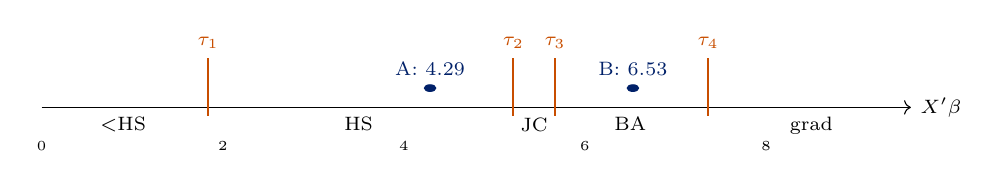
\begin{tikzpicture}[x=1.15cm,y=0.7cm]
  \draw[->] (0,0) -- (9.6,0) node[right]{\scriptsize $X'\beta$};
  \foreach \t/\l in {1.84/$\tau_1$,5.21/$\tau_2$,5.67/$\tau_3$,7.36/$\tau_4$}
    {\draw[accent,thick] (\t,-0.15) -- (\t,0.9); \node[accent,above] at (\t,0.9) {\scriptsize \l};}
  \node[below] at (0.9,0) {\scriptsize $<$HS};
  \node[below] at (3.5,0) {\scriptsize HS};
  \node[below] at (5.44,-0.02) {\scriptsize JC};
  \node[below] at (6.5,0) {\scriptsize BA};
  \node[below] at (8.5,0) {\scriptsize grad};
  \fill[dukeblue] (4.29,0.35) circle (0.07); \node[dukeblue,above] at (4.29,0.4) {\scriptsize A: $4.29$};
  \fill[dukeblue] (6.53,0.35) circle (0.07); \node[dukeblue,above] at (6.53,0.4) {\scriptsize B: $6.53$};
  \foreach \t in {0,2,4,6,8} \node[below,yshift=-9pt] at (\t,0) {\tiny \t};
\end{tikzpicture}
\end{center}
\vskip-4pt
$\Pr(Y_i \le j) = \Lambda(\tau_j - X_i'\bm\beta)$: the chance of being at
or below gate $j$ is the S-curve at the \emph{distance from the person to
the gate}. Each category's probability is the mass between two gates;
junior college is a narrow band, so it gets little mass for anyone.
\begin{center}\footnotesize
\renewcommand{\arraystretch}{1.0}
\begin{tabular}{lcccccc}
\toprule
 & $X'\hat\beta$ & $<$HS & HS & JC & BA & grad \\
\midrule
A: parents 12 yrs, vocabulary 5, male, white & $4.29$ & $0.08$ & $0.64$ & $0.08$ & $0.16$ & $0.04$ \\
B: parents 16 yrs, vocabulary 8, female, white & $6.53$ & $0.01$ & $0.20$ & $0.09$ & $0.40$ & $0.30$ \\
\bottomrule
\end{tabular}
\end{center}
\end{frame}

\begin{frame}{Reading an Ordered Logit: Five Probabilities Move\core}
A coefficient says the line moves; readers want the five probabilities.
Observed-value predictions, vocabulary $4$ versus $8$:
\begin{center}\small
\renewcommand{\arraystretch}{1.05}
\begin{tabular}{lccccc}
\toprule
 & $<$HS & HS & junior college & bachelor's & graduate \\
\midrule
vocabulary $= 4$ & $0.09$ & $0.59$ & $0.08$ & $0.18$ & $0.06$ \\
vocabulary $= 8$ & $0.03$ & $0.35$ & $0.10$ & $0.33$ & $0.19$ \\
\midrule
difference & $-0.07$ & $-0.24$ & $+0.02$ & $+0.16$ & $+0.14$ \\
\bottomrule
\end{tabular}
\end{center}
\vskip3pt
\begin{itemize}\itemsep2pt
  \item Four more words move a quarter of the population out of ``high
        school only,'' mostly into bachelor's and graduate degrees.
  \item The middle category barely moves: one $\hat\beta$ pushes
        probability \emph{through} a narrow band without piling it up. The
        sign of the effect on a middle category is not the sign of
        $\hat\beta$. (\texttt{avg\_predictions()} again.)
\end{itemize}
\end{frame}

\begin{frame}{Proportional Odds, and Checking It\core}
One $\bm\beta$ for every cutpoint is an assumption: vocabulary pushes
people past the HS line and the bachelor's line by the same log-odds.
Check it with four separate binary logits, ``above cut $j$'' versus not:
\begin{center}\small
\renewcommand{\arraystretch}{1.05}
\begin{tabular}{lcccc}
\toprule
above \dots & $<$HS & HS & junior college & bachelor's \\
\midrule
parents' education & $0.231$ & $0.198$ & $0.207$ & $0.180$ \\
vocabulary & $0.407$ & $0.348$ & $0.391$ & $0.331$ \\
female & $0.252$ & $0.367$ & $0.279$ & $0.379$ \\
\bottomrule
\end{tabular}
\end{center}
\vskip2pt
\begin{itemize}\itemsep1pt
  \item The ordered model's $0.358$ for vocabulary is a compromise between
        $0.33$ and $0.41$: proportional odds is a fair summary here.
  \item Formal check: LR against a multinomial logit on degree, which
        frees all four rows ($20$ parameters): $27.3$ on $12$ df,
        $p = 0.007$. Significant,
        as everything is at $n = 3{,}509$; the table says the violation is
        small. Judge the table, then the test; if it fails badly, free
        that covariate only (\texttt{ordinal::clm}).
\end{itemize}
\end{frame}

\begin{frame}{In the Literature: Multinomial Logit\core}
\textbf{Kuo and Raley (2016, \emph{Demography}).} What happens to a first
premarital cohabitation? Three outcomes in each month: it becomes a
marriage, it dissolves, or it continues. A discrete-time multinomial logit
on person-months from the National Survey of Family Growth, two cohorts.
\begin{itemize}\itemsep3pt
  \item Within three years: $41\%$ married and $35\%$ separated in the
        1990--95 cohort; $24\%$ married and $41\%$ separated in 2005--10.
  \item The retreat from marriage is educational: college-educated
        cohabitors' annual marriage probability held steady; for those
        without a degree it fell to less than half.
  \item Why not a logit on ``married or not'': the alternative to
        marriage shifted from staying together to breaking up.
\end{itemize}
\vskip2pt
\textbf{Breen and Jonsson (2000, \emph{ASR}).} Swedish educational careers as multinomial transitions: ``continue or
leave'' hides \emph{which} branch a student continues into.
\end{frame}

\begin{frame}{In the Literature: Ordered Logit\core}
\textbf{Zajacova, Huzurbazar, and Todd (2017, \emph{Social Science \&
Medicine}).} Self-rated health, five ordered categories from excellent to
poor, $N = 296{,}679$ adults in the National Health Interview Survey.
\begin{itemize}\itemsep3pt
  \item Ordered logits by age group, with the female coefficient read as
        an odds ratio on the odds of \emph{worse} health, the same at
        every cut.
  \item Ages 25--44: women's odds are $1.12$ times men's with demographic
        controls only, and $1.00$ once health conditions and
        socioeconomic status are added. Ages 65--84: $0.75$, women
        healthier.
  \item The design is exactly this section's: one $\beta$ per covariate,
        four cutpoints, and the same coefficient compared across models
        that add controls, which is where the proportional-odds check and
        the caution about comparing coefficients across models both
        matter.
\end{itemize}
\end{frame}

%%%%%%%%%%%%%%%%%%%%%%%%%%%%%%%%%%%%%%%%%%%%%%%%%%%%%%%%%%%%%%%%%%%%%%%%%%%%%%%
\section[Counts]{Count Outcomes}
%%%%%%%%%%%%%%%%%%%%%%%%%%%%%%%%%%%%%%%%%%%%%%%%%%%%%%%%%%%%%%%%%%%%%%%%%%%%%%%
\begin{frame}\sectionpage\end{frame}

\begin{frame}{Poisson Regression: Week 3's Poisson With $\theta_i = e^{X_i'\bm\beta}$\core}
Number of children, $n = 3{,}509$:
$Y_i \mid X_i \sim \text{Poisson}(\theta_i)$, $\log\theta_i = X_i'\bm\beta$.
\begin{center}\small
\renewcommand{\arraystretch}{1.05}
\begin{tabular}{lrrrl}
\toprule
 & $\hat\beta$ & SE & $e^{\hat\beta}$ & reading \\
\midrule
education (years) & $-0.045$ & $0.005$ & $0.956$ & $4.4\%$ fewer children per year \\
female & $0.009$ & $0.027$ & $1.01$ & no difference \\
black & $0.360$ & $0.035$ & $1.43$ & $43\%$ more \\
experience (years) & $0.012$ & $0.001$ & $1.01$ & $1.2\%$ more per year (age) \\
ever married & $0.947$ & $0.043$ & $2.58$ & $2.6$ times as many \\
\bottomrule
\end{tabular}
\end{center}
\vskip2pt
\begin{itemize}\itemsep2pt
  \item $e^{\hat\beta_j}$ multiplies the expected count, because
        $h = \exp$ turns adding into multiplying; a small $\hat\beta$ is
        about a percentage.
  \item \textbf{Exposure}\adv: counts over different windows (years observed,
        population at risk) model the \emph{rate}:
        \texttt{offset(log(exposure))}, a coefficient fixed at $1$.
  \item Why not OLS on $\log y$: $\log 0$ is undefined and $30\%$ have no
        children. The likelihood uses the counts themselves. What can go
        wrong is the variance, next.
\end{itemize}
\end{frame}

\begin{frame}{Overdispersion: the Poisson's One Strong Claim\core}
Week 3's Poisson has one parameter, so its variance is not free:
$\Var(Y_i \mid X_i) = \E[Y_i \mid X_i] = \theta_i$. Real counts almost
always vary more, because people differ in ways $X$ does not capture: some
are systematically more event-prone.
\begin{itemize}\itemsep3pt
  \item Raw: mean $1.60$, variance $2.11$. Conditional on $X$ the excess
        is smaller but there: \texttt{AER::dispersiontest} estimates
        $\Var = \theta_i(1 + 0.17)$, $z = 3.96$, $p < 0.0001$.
  \item That test uses only the Poisson fit: it asks whether the residual
        variance grows with the mean faster than the Poisson allows,
        without fitting any alternative.
  \item \textbf{Consequence}: coefficients stay about right (the mean is
        still right), but \alert{standard errors are too small}, here by
        about $7\%$, in other data by a factor of two or three.
\end{itemize}
\vskip3pt
Three repairs, next frame; all three leave $\hat{\bm\beta}$ nearly alone
and fix the SEs.
\end{frame}

\begin{frame}{Three Repairs, Three Beliefs About the Variance}
The Poisson standard error comes from the Poisson's variance claim,
$\Var(Y_i \mid X_i) = \theta_i$. Once that claim is false, the SE is wrong,
and each repair replaces the claim with a different one:
\begin{center}\footnotesize
\renewcommand{\arraystretch}{1.1}
\begin{tabular}{lll}
\toprule
Repair & Belief about $\Var(Y_i \mid X_i)$ & What changes \\
\midrule
Quasi-Poisson & $\phi\,\theta_i$, one multiple everywhere & every SE, by one factor $\sqrt{\hat\phi}$ \\
Negative binomial & $\theta_i + \theta_i^2/\alpha$, grows faster than the mean & the likelihood: $\hat{\bm\beta}$ and SEs \\
Robust (sandwich) & none; use the squared residuals as they are & SEs only, each on its own \\
\bottomrule
\end{tabular}
\end{center}
\vskip2pt
\begin{itemize}\itemsep2pt
  \item All three leave $\hat{\bm\beta}$ essentially where the Poisson
        put it: the mean is not in question, only the scatter around it.
  \item They differ in how much they assume: one number, a particular
        shape, or nothing (paid for with noisier SEs).
\end{itemize}
Next: the arithmetic behind each number for one coefficient, \emph{ever
married}, whose Poisson SE is $0.0430$.
\end{frame}

\begin{frame}{Where the Three Numbers Come From}
\begin{itemize}\itemsep4pt
  \item \textbf{Quasi-Poisson, $0.0461$.} $\hat\phi = \frac{1}{n-k}\sum_i
        (y_i - \hat\theta_i)^2/\hat\theta_i = 1.149$: under the Poisson
        each term averages $1$; the counts scatter $15\%$ more. Multiply
        every Poisson SE by $\sqrt{1.149} = 1.072$:
        $0.0430 \times 1.072 = 0.0461$. Nothing else moves.
  \item \textbf{Negative binomial, $0.0437$.} A new likelihood with
        variance $\theta_i + \theta_i^2/\alpha$; the data choose
        $\hat\alpha = 31$, so at the mean count $1.6$ the variance is
        $1.68$, not $1.60$. Each observation's weight in the curvature
        falls by the factor $1/(1 + \theta_i/\hat\alpha) \approx 0.95$, and
        the SE grows by about $2\%$. Mild, because $\hat\alpha$ is large.
  \item \textbf{Robust, $0.0551$.} Week 2's sandwich,
        $(X'WX)^{-1}\big[\sum_i X_iX_i'(y_i - \hat\theta_i)^2\big](X'WX)^{-1}$,
        uses each person's own squared residual. Why so much larger here:
        the excess scatter is not uniform. Among the never married the
        Pearson ratio is $1.66$, among the ever married $0.96$. One
        $\hat\phi = 1.15$ averages them; the sandwich sees that this
        dummy compares exactly the two groups whose scatter differs.
\end{itemize}
\end{frame}

\begin{frame}{Excess Zeros\core}
\begin{columns}[c]
\begin{column}{0.52\textwidth}
\centering
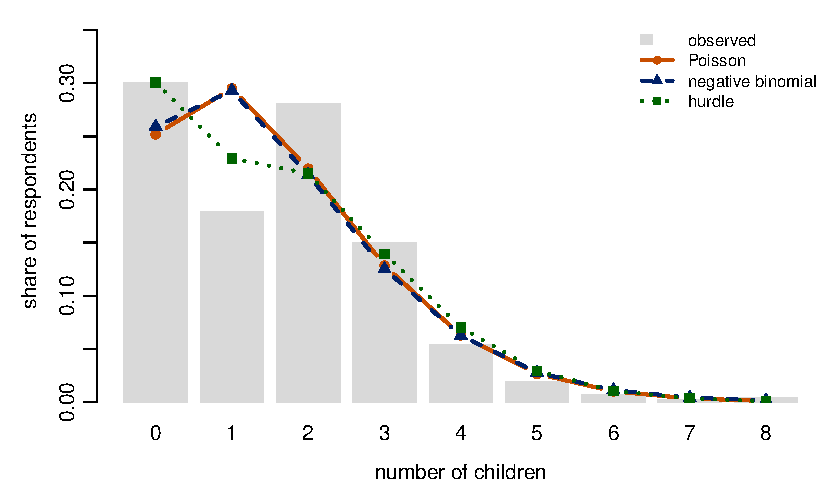
\includegraphics[width=\linewidth]{figs/childs_dist.pdf}
\end{column}
\begin{column}{0.46\textwidth}
\begin{itemize}\itemsep3pt
  \item Observed: $30\%$ childless. Poisson predicts $25\%$, the negative
        binomial $26\%$. Neither has a way to make zeros special.
  \item Sociologically zero \emph{is} special: whether to have children
        and how many are different decisions. Two models that say so:
\end{itemize}
\end{column}
\end{columns}
\begin{itemize}\itemsep2pt
  \item \textbf{Hurdle}: a logit for zero versus positive, then a
        \emph{truncated} count model for the positives. \texttt{pscl::hurdle}.
  \item \textbf{Zero-inflated}: a mixture; a share of ``structural
        zeros'' who could never have a positive count, the rest a count
        model that can also produce zeros. \texttt{pscl::zeroinfl}.
\end{itemize}
\end{frame}

\begin{frame}{The Hurdle Model on the GSS\core}
\vskip-2pt
Same five covariates in both parts; count part Poisson.
\begin{center}\small
\renewcommand{\arraystretch}{0.95}
\begin{tabular}{lcc@{\qquad}cc}
\toprule
 & \multicolumn{2}{c}{\textbf{any children?} (logit)} & \multicolumn{2}{c}{\textbf{how many, given some} (Poisson)} \\
 & $\hat\beta$ & $e^{\hat\beta}$ & $\hat\beta$ & $e^{\hat\beta}$ \\
\midrule
education & $-0.116$ & $0.89$ & $-0.037$ & $0.96$ \\
female & $0.294$ & $1.34$ & $-0.074$ & $0.93$ \\
black & $1.071$ & $2.92$ & $0.225$ & $1.25$ \\
ever married & $2.187$ & $8.91$ & $0.298$ & $1.35$ \\
\bottomrule
\end{tabular}
\end{center}
\vskip2pt
\begin{itemize}\itemsep2pt
  \item Two processes: marriage multiplies the odds of \emph{any} child
        by $9$ but the count among parents by $1.35$; women are likelier
        to have any child and have slightly fewer. One Poisson averaged these.
  \item Fit: $\loglik$ rises from $-5{,}383$ (Poisson) to $-5{,}228$,
        AIC $10{,}778 \to 10{,}479$, six more parameters. Zeros matched exactly.
\end{itemize}
\end{frame}

\begin{frame}{Which Count Model, and How to Decide\core}
\begin{enumerate}\itemsep4pt
  \item Start with \textbf{Poisson, robust SEs}. Coefficients are right for
        the mean under any variance; $e^{\hat\beta}$ is the cleanest
        reading in the deck.
  \item Run the \textbf{overdispersion test}. If it rejects and
        you need a likelihood (prediction, AIC, LR against a bigger
        model), fit the \textbf{negative binomial}.
  \item Compare the \textbf{observed and predicted distribution} of counts,
        as in the figure. A zero problem is visible before any test.
  \item \textbf{Hurdle or zero-inflated}: choose on substance. Hurdle when
        crossing from zero to one is a different \emph{process}
        (having any children, ever being arrested). Zero-inflated when
        some zeros are a different \emph{kind} of person (a nonsmoker's
        zero cigarettes versus a smoker's zero today). Then AIC or BIC
        between them; they are not nested.
  \item Never compare by fit alone across models fitted to different rows.
\end{enumerate}
\end{frame}

\begin{frame}{In the Literature: Negative Binomial\core}
\textbf{Olzak (2021, \emph{ASR}).} Officer-involved fatalities of Black,
Latino, and white residents, counted per city-year in the $170$ largest
U.S.\ cities. Many city-years have zero and the variance far exceeds the
mean, so negative binomial rather than Poisson.
\begin{itemize}\itemsep3pt
  \item One local protest against police brutality is followed by $11\%$
        fewer Black fatalities and $7\%$ fewer Latino fatalities the next
        year ($e^{\hat\beta} - 1$, read as a percent), and no change for
        whites.
  \item The count model is doing what the section said: the mean is right
        under the Poisson too, but the standard errors would be badly
        too small.
\end{itemize}
\end{frame}

\begin{frame}{In the Literature: Excess Zeros\core}
\textbf{Ajrouch, Antonucci, and Webster (2016, \emph{Journals of
Gerontology: Series B}).} Hours volunteered, two waves, $n = 543$; most
respondents report zero.
\begin{itemize}\itemsep3pt
  \item A zero-inflated negative binomial: a logit for being a
        never-volunteer, and a negative binomial for hours that can also
        give a zero (a volunteer with no hours this wave).
  \item The authors read the two equations as \emph{whether} and
        \emph{how much}, which is the hurdle's reading: network proximity
        and contact predict whether; education predicts how much.
  \item Strictly, only the hurdle splits zeros from positives that
        cleanly. In practice the two give similar coefficients and are
        read the same way; they differ only in what a zero may mean, and
        the data rarely say which.
\end{itemize}
\vskip2pt
\textbf{Where you will see these.} Health, criminology, gerontology. In
\emph{ASR} and \emph{AJS} a negative binomial with robust SEs usually
carries the day. Use a two-part model when zero is a different kind of
answer, not because zeros are many.
\end{frame}

%%%%%%%%%%%%%%%%%%%%%%%%%%%%%%%%%%%%%%%%%%%%%%%%%%%%%%%%%%%%%%%%%%%%%%%%%%%%%%%
\section[Multilevel]{Multilevel Models}
%%%%%%%%%%%%%%%%%%%%%%%%%%%%%%%%%%%%%%%%%%%%%%%%%%%%%%%%%%%%%%%%%%%%%%%%%%%%%%%
\begin{frame}\sectionpage\end{frame}

\begin{frame}{Observations Come in Groups\core}
Often the question is about a group's characteristic as much as the
individual's: does a Catholic school raise achievement net of who attends it
(Coleman, Hoffer, and Kilgore 1982)? The intuitive move: put both kinds of
variable in one OLS. High School and Beyond, $7{,}185$ students, $160$ schools:
\begingroup
\setlength{\abovedisplayskip}{2pt}\setlength{\belowdisplayskip}{2pt}
\begin{align*}
  \text{math}_{ij} = \beta_0 + \beta_1\,\text{SES}_{ij}
  + \beta_2\,\text{Catholic}_j + e_{ij},
  \qquad \hat\beta_2 = 1.94,\ \text{SE}\ 0.15.
\end{align*}
\endgroup
\begin{alertblock}{What is wrong}
Catholic takes $160$ values, not $7{,}185$. Students in the same school share
what the model left out about it, so their errors are correlated and OLS counts
each school's evidence many times over. The clustered SE (Week 2) is $0.32$,
twice the OLS one.
\end{alertblock}
\end{frame}

\begin{frame}{Why Not Just OLS With Clustered Standard Errors?\core}
Week 2 split the OLS error into a group shock and a personal one,
$\epsilon_{ig} = \nu_g + \eta_{ig}$. Same split, school as the cluster,
$u_j$ for $\nu_g$:
\begingroup
\setlength{\abovedisplayskip}{2pt}\setlength{\belowdisplayskip}{2pt}
\begin{align*}
  \text{math}_{ij} = \beta_0 + \beta_1\,\text{SES}_{ij}
  + \beta_2\,\text{Catholic}_j + u_j + e_{ij}.
\end{align*}
\endgroup
$u_j$: how far school $j$ sits above or below the average school once SES
and sector are accounted for, the same for every student in it; $e_{ij}$ is
the student's own deviation. Three things to do with $u_j$:
\begin{itemize}\itemsep1pt
  \item \textbf{Clustered OLS} (Week 2) used the split only to see what was
        wrong, then repaired the SEs without estimating $u_j$ or its variance.
  \item \textbf{Fixed effects} (Week 10) estimate every $u_j$: $160$
        dummies. Catholic does not vary within a school, so it is absorbed.
  \item \textbf{This week} treats the $u_j$ as draws from a distribution and
        estimates their \emph{variance}. Catholic stays estimable, and the
        variance answers what neither of the others can: how much variation
        is between schools? Here $18\%$, Coleman et al.'s (1966) question.
\end{itemize}
\end{frame}

\begin{frame}{The Random-Intercept Model\core}
Student $i$ in school $j$, the equation from the last frame with the
distributions filled in:
\begin{align*}
  \text{math}_{ij} = \beta_0 + \beta_1\,\text{SES}_{ij} + \beta_2\,\text{Catholic}_j + u_j + e_{ij},
  \qquad u_j \sim \mathcal N(0, \tau^2), \quad e_{ij} \sim \mathcal N(0, \sigma^2).
\end{align*}
\begin{itemize}\itemsep3pt
  \item Each school has its own intercept, $\beta_0 + u_j$. Fixed effects
        would estimate the $160$ shifts as $160$ constants; here they are
        $160$ draws from one distribution, and its variance $\tau^2$ is what
        gets estimated.
  \item Two students in the same school share $u_j$, so
        $\Cov(\text{math}_{ij}, \text{math}_{i'j}) = \tau^2$ and
        $\Var(\text{math}_{ij}) = \tau^2 + \sigma^2$. The model \emph{is} the
        correlation clustering corrects for.
  \item Parameters: $\beta_0, \beta_1, \beta_2, \tau^2, \sigma^2$. Five,
        whatever the number of schools. Fixed effects would need $162$ and
        could not include Catholic.
\end{itemize}
\vskip3pt
\textbf{Estimation.} $u_j$ is never observed, so each school's likelihood
averages over the values it could take; Newton maximizes the result in
$(\bm\beta, \tau^2, \sigma^2)$.
\texttt{lme4::lmer(math \~{} ses + catholic + (1 | school))}.
\end{frame}

\begin{frame}{Reading the Fit, and the Intraclass Correlation\core}
\begin{columns}[c]
\begin{column}{0.46\textwidth}
\centering\small
\renewcommand{\arraystretch}{1.05}
\begin{tabular}{lcc}
\toprule
 & estimate & SE \\
\midrule
intercept $\hat\beta_0$ & $11.72$ & $0.23$ \\
SES $\hat\beta_1$ & $2.38$ & $0.11$ \\
Catholic $\hat\beta_2$ & $2.10$ & $0.34$ \\
between schools $\hat\tau^2$ & $3.62$ & \\
within schools $\hat\sigma^2$ & $37.0$ & \\
\bottomrule
\end{tabular}
\end{column}
\begin{column}{0.52\textwidth}
\begin{itemize}\itemsep1pt
  \item $\hat\beta$: as in any regression. A unit of SES adds $2.4$
        points; a Catholic school adds $2.1$ at the same SES.
  \item $\hat\tau^2$: schools of the same sector with the same SES
        students still differ, SD $\sqrt{3.62} = 1.9$ points.
  \item $\hat\sigma^2$: classmates differ from their school's line by
        SD $\sqrt{37.0} = 6.1$ points.
\end{itemize}
\end{column}
\end{columns}
\vskip2pt
\begin{itemize}\itemsep1pt
  \item $\text{ICC} = \hat\tau^2/(\hat\tau^2 + \hat\sigma^2) = 3.62/40.6
        = 0.09$: of the variation SES and sector leave unexplained, $9\%$ is
        between schools; two classmates of the same SES correlate at
        $0.09$, Week 2's $\rho_e$ now estimated. Is $\tau^2$ zero? LR
        against OLS with the same $x$: $332$.
  \item With no predictors: $\hat\tau^2 = 8.55$, $\hat\sigma^2 = 39.15$,
        ICC $= 0.18$, the raw split. SES and sector cut the between-school
        variance by $58\%$, the within-school by $5\%$.
\end{itemize}
\end{frame}

\begin{frame}{Shrinkage: What the Model Says About One School\core}
With no predictors, the model's estimate of school $j$'s mean is a weighted
average of the school's own mean and the grand mean $12.64$:
\begin{align*}
  \hat\mu_j = w_j\,\bar y_j + (1 - w_j)\,\hat\beta_0,
  \qquad
  w_j = \frac{n_j\,\tau^2}{n_j\,\tau^2 + \sigma^2}.
\end{align*}
\begin{center}\small
\renewcommand{\arraystretch}{1.05}
\begin{tabular}{lcccc}
\toprule
school & $n_j$ & own mean $\bar y_j$ & weight $w_j$ & model estimate $\hat\mu_j$ \\
\midrule
smallest & $14$ & $4.55$ & $0.75$ & $6.54$ \\
largest & $67$ & $11.14$ & $0.94$ & $11.23$ \\
\bottomrule
\end{tabular}
\end{center}
\begin{itemize}\itemsep3pt
  \item A $14$-student mean is noisy, so the model pulls it a quarter of
        the way toward $12.64$; a $67$-student mean is nearly left alone.
  \item The weight rises with $n_j$ and with $\tau^2/\sigma^2$: the more
        schools differ, the more each school's own mean counts.
  \item Week 12's ridge shrinkage, arrived at by likelihood.
\end{itemize}
\end{frame}

\begin{frame}{Predictors at Both Levels\core}
Student SES (level 1) and school sector, Catholic versus public (level 2):
\begin{center}\small
\renewcommand{\arraystretch}{1.05}
\begin{tabular}{lcccc}
\toprule
 & pooled OLS & OLS, clustered SE & random intercept & fixed effects \\
\midrule
SES & $2.95$ ($0.10$) & $2.95$ ($0.13$) & $2.38$ ($0.11$) & $2.19$ ($0.11$) \\
Catholic & $1.94$ ($0.15$) & $1.94$ ($0.32$) & $2.10$ ($0.34$) & not identified \\
$\hat\tau^2$, $\hat\sigma^2$ & & & $3.62$, $37.0$ & \\
\bottomrule
\end{tabular}
\end{center}
\begin{itemize}\itemsep3pt
  \item \textbf{Sector} is constant within school. Fixed effects absorb
        it; only a model with a between-school variance can estimate it:
        Catholic schools score $2.1$ points higher, SE $0.34$ with $160$
        schools as the units.
  \item \textbf{SES} falls from $2.95$ to $2.38$ to $2.19$ as schools go
        from ignored to modelled to conditioned on: part of the pooled
        slope is high-SES students attending high-scoring schools.
  \item $\hat\tau^2$ fell from $8.55$ to $3.62$: SES and sector explain
        $58\%$ of the between-school variance.
\end{itemize}
\end{frame}

\begin{frame}{Fixed or Random?\core}
\begin{center}\small
\renewcommand{\arraystretch}{1.15}
\begin{tabular}{lll}
\toprule
 & Fixed effects (Week 10) & Random intercept \\
\midrule
group differences & $J$ dummies & one variance $\tau^2$ \\
assumption & none about $u_j$ & $u_j$ uncorrelated with $x_{ij}$ \\
group-level $x$ & impossible & estimable \\
few units per group & noisy & shrinkage helps \\
answers & within-group effect of $x$ & both levels; how much is between \\
\bottomrule
\end{tabular}
\end{center}
\vskip3pt
\begin{itemize}\itemsep3pt
  \item The assumption that matters: if high-$u_j$ schools also have
        high-SES students, the random-intercept SES slope is biased. Here
        $2.38$ against $2.19$, a small violation.
  \item \textbf{Practice}: a causal question about a within-group
        variable, fixed effects. A group-level variable, or the groups
        themselves, random intercept. Never plain OLS SEs.
\end{itemize}
\end{frame}

\begin{frame}{Random-Intercept Logit, and \texttt{R}\core}
Binary outcome, top quartile of the math score:
$\Pr(y_{ij} = 1) = \Lambda(\beta_0 + \beta_1 x_{ij} + u_j)$, $u_j \sim
\mathcal N(0, \tau^2)$. Week 4's logit with a school shift.
\begin{center}\small
\renewcommand{\arraystretch}{1.0}
\begin{tabular}{lcc}
\toprule
 & $\hat\beta$ & SE \\
\midrule
SES & $0.674$ & $0.045$ \\
Catholic & $0.391$ & $0.112$ \\
$\hat\tau^2$ & $0.34$ & \\
\bottomrule
\end{tabular}
\end{center}
\begin{itemize}\itemsep3pt
  \item No closed form for the integral over $u_j$:
        \texttt{glmer(..., family = binomial, nAGQ = 10)} does it
        numerically, slower, and can fail to converge.
  \item Coefficients are within-school. For population-average
        probabilities, average predictions over $u_j$.
  \item \texttt{lmer}/\texttt{glmer} print $\hat\tau$ as ``Std.Dev.'';
        square it. Random slopes: \texttt{(1 + x | school)}.
\end{itemize}
\end{frame}

\begin{frame}{In the Literature: Multilevel\core}
\textbf{Sampson, Raudenbush, and Earls (1997, \emph{Science}), ``Neighborhoods
and Violent Crime.''} $8{,}782$ residents in $343$ Chicago neighborhoods.
\begin{itemize}\itemsep3pt
  \item Level 1: residents' reports of cohesion and willingness to
        intervene, adjusted for individual characteristics. Level 2: the
        neighborhood intercept, $u_j$, is the neighborhood's
        \emph{collective efficacy}. The between-neighborhood variance is
        what makes it a neighborhood property rather than a respondent's
        opinion.
  \item Collective efficacy is negatively associated with violence, and
        it mediates most of the association of concentrated disadvantage
        and residential instability with violence.
  \item The paper's method is the one on these frames: a random intercept
        per neighborhood, its reliability from $\tau^2$, $\sigma^2$, and
        $n_j$, and neighborhood-level predictors that fixed effects could
        not estimate.
\end{itemize}
\vskip3pt
The textbook: Raudenbush and Bryk (2002), whose running example is the
High School and Beyond data used here.
\end{frame}

%%%%%%%%%%%%%%%%%%%%%%%%%%%%%%%%%%%%%%%%%%%%%%%%%%%%%%%%%%%%%%%%%%%%%%%%%%%%%%%
\section[Event History]{Event History (Survival) Analysis}
%%%%%%%%%%%%%%%%%%%%%%%%%%%%%%%%%%%%%%%%%%%%%%%%%%%%%%%%%%%%%%%%%%%%%%%%%%%%%%%
\begin{frame}\sectionpage\end{frame}

\begin{frame}{Durations Are Different\core}
Time-to-event outcomes: age at first birth, time to marriage or divorce, job
tenure, time to reoffending, organizational survival.
\vskip2pt
\begin{alertblock}{The defining problem: censoring}
For many units the clock is still running when observation ends: a respondent
aged 35 without a child is not a ``no,'' she is a \emph{not yet}. We observe
$\min(T_i, C_i)$ plus an indicator $\delta_i$ for whether the event was seen.
\end{alertblock}
\begin{itemize}\itemsep2pt
  \item Dropping censored cases selects on the outcome; coding them as
        event-free forever understates durations. Both bias.
  \item The fix is this week's principle: \alert{write down the probability of
        exactly what you observed}, censoring included.
\end{itemize}
\end{frame}

\begin{frame}{The Two Building Blocks: Survival and Hazard\core}
For a duration $T$ with density $f(t)$:
\begin{align*}
  S(t) = \Pr(T > t)
  \qquad\text{and}\qquad
  h(t) = \frac{f(t)}{S(t)} .
\end{align*}
\begin{itemize}\itemsep3pt
  \item $S(t)$, the \textbf{survival function}: the share still event-free at
        $t$. Starts at 1, never rises.
  \item $h(t)$, the \textbf{hazard}: the event \emph{rate} at $t$ among those
        still at risk, the chance of a first birth at age 30 \emph{given}
        childless at 30. This conditional rate is what sociological theory is
        usually about.
  \item Either determines the other; models are written on the hazard scale.
\end{itemize}
\end{frame}

\begin{frame}{The Likelihood That Censoring Demands\core}
Each unit contributes the probability of what we actually saw:
\begin{itemize}\itemsep2pt
  \item event observed at $t_i$ ($\delta_i = 1$): contribute the density
        $f(t_i)$;
  \item censored at $t_i$ ($\delta_i = 0$): contribute
        $S(t_i) = \Pr(T > t_i)$, the probability of lasting past the point
        where we lost sight of them.
\end{itemize}
\begin{align*}
  \lik = \prod_{i=1}^{n} f(t_i)^{\delta_i}\, S(t_i)^{1-\delta_i}
  \qquad\Longrightarrow\qquad
  \loglik = \sum_i \Big[\delta_i \log f(t_i) + (1-\delta_i)\log S(t_i)\Big] .
\end{align*}
\vskip2pt
Censored units are neither dropped nor mislabelled; each contributes exactly
the information it carries. Least squares has no way to write this down.
\end{frame}

\begin{frame}{Kaplan--Meier: $S(t)$ Without a Model\core}
Order the observed event times $t_{(1)} < t_{(2)} < \cdots$; let $n_j$ be the
number still at risk just before $t_{(j)}$ and $d_j$ the number of events
there:
\begin{align*}
  \hat S(t) = \prod_{j:\, t_{(j)} \leq t} \left(1 - \frac{d_j}{n_j}\right) .
\end{align*}
\begin{itemize}\itemsep2pt
  \item Read it as a chain of conditional survivals: to be event-free at $t$
        you must get past each earlier event time, and $1 - d_j/n_j$ estimates
        each step.
  \item Censored units sit in the risk sets $n_j$ while observed, then leave:
        their partial information is used, then released.
  \item The step-function plot of $\hat S(t)$, by group, is the field's
        standard descriptive. Look at it before any model.
\end{itemize}
\end{frame}

\begin{frame}{The Cox Proportional-Hazards Model\core}
Put covariates on the hazard, multiplicatively:
\begin{align*}
  h(t \mid X_i) = h_0(t)\, \exp\!\big(X_i'\bm\beta\big) .
\end{align*}
\begin{itemize}\itemsep3pt
  \item $h_0(t)$, the \textbf{baseline hazard}, is left completely
        unspecified: no claim about \emph{when} events happen, only about how
        covariates scale the rate.
  \item $e^{\beta_j}$ is a \alert{hazard ratio}: $e^{\beta_j} = 1.3$ means a
        30\% higher event rate at every moment, per unit of $X_j$.
  \item Estimation\adv: the \emph{partial likelihood} compares, at each event
        time, the unit that failed with everyone still at risk; $h_0(t)$
        cancels out of every comparison \srcp{Cox 1972}.
  \item The name is the assumption: \alert{proportional} hazards, a constant
        ratio between any two units over time. Check it
        (\texttt{cox.zph}) rather than assume it.
\end{itemize}
\end{frame}

\begin{frame}{Discrete Time: Event History as the Logit You Already Know\core}
Sociological clocks are usually discrete (ages, years, waves), and a standard
construction reduces event history to this week's tools \srcp{Allison 2014}:
\begin{enumerate}\itemsep2pt
  \item Expand to \textbf{person-period} data: one row per unit per period at
        risk (childless person-years, employed person-months).
  \item Outcome $=1$ in the period the event occurs, $0$ otherwise; a unit's
        rows stop at its event or its censoring.
  \item Run a \alert{logit} of the outcome on covariates plus period dummies,
        which act as a nonparametric baseline hazard.
\end{enumerate}
\vskip2pt
\begin{itemize}\itemsep2pt
  \item The coefficients are discrete-time (log) hazard ratios, and
        time-varying covariates enter for free, updated row by row.
  \item Censoring is handled by construction: censored units simply stop
        contributing rows, the likelihood logic from three frames back.
\end{itemize}
\end{frame}

\begin{frame}{In the Literature: Discrete-Time Event History\core}
\textbf{Killewald (2016, \emph{ASR}).} ``Money, Work, and Marital
Stability.'' Does a wife's economic independence, or a husband's failure to
provide, raise the risk of divorce, and has that changed? Couples in the
Panel Study of Income Dynamics, 1968--2013, followed year by year.
\begin{itemize}\itemsep3pt
  \item Person-year data and a logit on ``divorced this year,'' covariates
        updated each year: the construction on the previous frame. Couples
        still married when observation ends are censored, not ``never
        divorced.''
  \item For marriages begun after 1975, a husband not employed full-time
        raises the predicted probability of divorce in the following year
        from $2.5\%$ to $3.3\%$; neither the wife's full-time employment nor
        her share of the housework predicts divorce.
  \item Why not a logit on ``ever divorced'': couples are observed for
        different lengths, and the risk each year is the quantity the theory
        is about.
\end{itemize}
\end{frame}

\begin{frame}{Event History in \texttt{R}, and What to Watch}
\begin{itemize}\itemsep3pt
  \item \texttt{survival::Surv(time, event)} builds the outcome;
        \texttt{survfit()} gives Kaplan--Meier; \texttt{coxph()} fits the Cox
        model; \texttt{cox.zph()} checks proportionality.
  \item Discrete time: build the person-period data
        (\texttt{survSplit()}), then plain \texttt{glm(..., binomial)}.
        Everything from this week applies, marginal effects included; cluster
        standard errors on the person.
  \item \textbf{Watch for}: informative censoring (dropout related to event
        risk breaks the likelihood); left truncation (late entry to the risk
        set); unobserved heterogeneity (``frailty'') making hazards look
        spuriously declining. Allison (2014) covers all three.
\end{itemize}
\end{frame}

%%%%%%%%%%%%%%%%%%%%%%%%%%%%%%%%%%%%%%%%%%%%%%%%%%%%%%%%%%%%%%%%%%%%%%%%%%%%%%%
\section[Practice]{Diagnostics and Practice}
%%%%%%%%%%%%%%%%%%%%%%%%%%%%%%%%%%%%%%%%%%%%%%%%%%%%%%%%%%%%%%%%%%%%%%%%%%%%%%%
\begin{frame}\sectionpage\end{frame}

\begin{frame}{Assessing Fit}
\begin{itemize}\itemsep2pt
  \item \textbf{Deviance} $= 2\big(\loglik_{\text{saturated}} - \loglik_{\text{fitted}}\big)$:
        the GLM analogue of the residual sum of squares. The saturated term is
        common to nested models, so \emph{differences} in deviance are exactly LR
        tests. Non-nested models: AIC and BIC (first section).
  \item \textbf{Pseudo-$R^2$} (McFadden: $1 - \loglik_{\text{full}}/\loglik_{\text{null}}$):
        a rank ordering, not ``variance explained''; $0.2$--$0.4$ counts as
        excellent.
  \item \textbf{Classification accuracy} needs a threshold and misleads with
        rare outcomes: compare against always predicting the majority class.
        \textbf{AUC} averages over thresholds: $0.5$ is a coin flip.
  \item \textbf{Predictive checks}: simulate outcomes from the fitted model
        and compare to the data. Most informative, least used.
\end{itemize}
\end{frame}

\begin{frame}{A Practical Protocol\core}
\begin{enumerate}\itemsep4pt
  \item Choose the distribution from the \emph{outcome}, and the link from
        convention. Do not agonize over logit versus probit.
  \item Fit, then check convergence and look for separation.
  \item Check overdispersion for counts; check proportional odds for ordered
        outcomes.
  \item \alert{Report average marginal effects or predicted probabilities}, with
        intervals from the delta method or simulation. Coefficient tables belong
        in an appendix.
  \item Never compare raw coefficients across nested logit models or across
        groups. Compare marginal effects.
  \item Cluster whenever the design has clusters (Week 2). For counts,
        robust standard errors as a matter of course. For a logit, a large gap
        between robust and model-based standard errors is a warning that the
        model is wrong, not a fix: repair the model.
\end{enumerate}
\end{frame}

\begin{frame}{Looking Ahead}
\begin{itemize}\itemsep5pt
  \item Both estimation engines are now in hand: least squares and maximum
        likelihood. The rest of the course applies one of them to a
        well-chosen quantity.
  \item \alert{Nothing in Weeks 1--4 says a coefficient is a causal effect.}
        We have been describing conditional distributions.
  \item \textbf{Week 5} changes the question: potential outcomes and DAGs say
        what we \emph{want} to estimate and what must hold to get it.
\end{itemize}
\vskip6pt
\begin{block}{Problem Set 2}
Assigned today, due Monday September 28. Covers Weeks 3--4: deriving and coding
likelihoods, information and standard errors, and interpreting limited dependent
variable models on the GSS.
\end{block}
\end{frame}

\begin{frame}[allowframebreaks,t]{References}
\footnotesize
\begin{itemize}\itemsep3pt
\item Ai, Chunrong and Edward C. Norton. 2003. ``Interaction Terms in Logit and
Probit Models.'' \textit{Economics Letters} 80(1): 123--129.
\item Allison, Paul D. 1999. ``Comparing Logit and Probit Coefficients Across
Groups.'' \textit{Sociological Methods \& Research} 28(2): 186--208.
\item Allison, Paul D. 2014. \textit{Event History and Survival Analysis},
2nd ed. Sage.
\item Berry, William D., Jacqueline H.R. DeMeritt, and Justin Esarey. 2010.
``Testing for Interaction in Binary Logit and Probit Models: Is a Product Term
Essential?'' \textit{American Journal of Political Science} 54(1): 248--266.
\item Cox, D.R. 1972. ``Regression Models and Life-Tables.'' \textit{Journal
of the Royal Statistical Society, Series B} 34(2): 187--220.
\item Hanmer, Michael J. and Kerem Ozan Kalkan. 2013. ``Behind the Curve:
Clarifying the Best Approach to Calculating Predicted Probabilities and Marginal
Effects from Limited Dependent Variable Models.''
\textit{American Journal of Political Science} 57(1): 263--277.
\item James, Gareth et al. 2021. \textit{An Introduction to Statistical Learning},
2nd ed. Springer. [Ch.\ 4]
\item King, Gary, Michael Tomz, and Jason Wittenberg. 2000. ``Making the Most of
Statistical Analyses: Improving Interpretation and Presentation.''
\textit{American Journal of Political Science} 44(2): 347--361.
\item Long, J. Scott. 1997. \textit{Regression Models for Categorical and Limited
Dependent Variables}. Sage. [the standard sociological reference]
\item Raftery, Adrian E. 1995. ``Bayesian Model Selection in Social
Research.'' \textit{Sociological Methodology} 25: 111--163.
\item Mood, Carina. 2010. ``Logistic Regression: Why We Cannot Do What We Think We
Can Do, and What We Can Do About It.'' \textit{European Sociological Review}
26(1): 67--82.
\item Zorn, Christopher. 2005. ``A Solution to Separation in Binary Response
Models.'' \textit{Political Analysis} 13: 157--170.
\item Ajrouch, Kristine J., Toni C. Antonucci, and Noah J. Webster. 2016.
``Volunteerism: Social Network Dynamics and Education.'' \textit{Journals of
Gerontology: Series B} 71(2): 309--319.
\item Breen, Richard and Jan O. Jonsson. 2000. ``Analyzing Educational Careers:
A Multinomial Transition Model.'' \textit{American Sociological Review} 65(5):
754--772.
\item Coleman, James S., Ernest Q. Campbell, Carol J. Hobson, James McPartland,
Alexander M. Mood, Frederic D. Weinfeld, and Robert L. York. 1966.
\textit{Equality of Educational Opportunity}. Washington, DC: U.S. Government
Printing Office.
\item Coleman, James S., Thomas Hoffer, and Sally Kilgore. 1982. \textit{High
School Achievement: Public, Catholic, and Private Schools Compared}. New York:
Basic Books.
\item Killewald, Alexandra. 2016. ``Money, Work, and Marital Stability:
Assessing Change in the Gendered Determinants of Divorce.'' \textit{American
Sociological Review} 81(4): 696--719.
\item Kuo, Janet Chen-Lan and R. Kelly Raley. 2016. ``Diverging Patterns of
Union Transition among Cohabitors by Race-Ethnicity and Education.''
\textit{Demography} 53(4): 921--935.
\item Olzak, Susan. 2021. ``Does Protest Against Police Violence Matter?
Evidence from U.S. Cities, 1990 through 2019.'' \textit{American Sociological
Review}, doi:10.1177/00031224211056966.
\item Pager, Devah. 2003. ``The Mark of a Criminal Record.'' \textit{American
Journal of Sociology} 108(5): 937--975.
\item Raudenbush, Stephen W. and Anthony S. Bryk. 2002. \textit{Hierarchical
Linear Models: Applications and Data Analysis Methods}, 2nd ed. Sage.
\item Sampson, Robert J., Stephen W. Raudenbush, and Felton Earls. 1997.
``Neighborhoods and Violent Crime: A Multilevel Study of Collective
Efficacy.'' \textit{Science} 277(5328): 918--924.
\item Zajacova, Anna, Snehalata Huzurbazar, and Megan Todd. 2017. ``Gender and
the Structure of Self-Rated Health across the Adult Life Span.'' \textit{Social
Science \& Medicine} 187: 58--66.
\end{itemize}
\end{frame}

\end{document}
